\chapter{Grundlagen}\label{grundlagen}

\section{Ballistokardiographie}

Die vorliegende Arbeit beschäftigt sich mit der Beurteilung der Signalqualität in ballistokardiographischen Signalen. Zum Verständnis der gemessenen Vorgänge und der Problematik in Bezug auf die Signalqualität und dessen Beurteilung ist grundlegendes medizinisches Wissen und messtechnisches Verständnis nötig. Aufgrund dessen wird hier eine kurze Übersicht über die medizinischen Grundlagen gegeben und die \acl{BKG} eingeführt.
	\subsection{Medizinische Grundlagen}
	
	\begin{itemize}
		\item Kardiorespiratorisches System
			\begin{itemize}
				\item Kardiorespiratorisches System besteht aus 2 Teilsystem: kardiovaskulär und respiratorisches System
				\item kardivaskulär: Herz, Arterien (sauerstoffreiches Blut), Venen (sauerstoffarmes Blut zur Anreicherung mit Sauerstoff zur Lunge)
				\item von Lungen in linke Herzkammer und durch Arterien zu Organen (Sauerstoff löst sich vom Blut)
				\item durch Venen zurück in rechte Herzkammer
				\item Zyklus beendet
				\item Vitalparameter: Herzfrequenz
				\item Herzschlag besteht aus 2 Phasen: füllende und auswerfende Phase
				\item Diastole (Erschlaffungs- und Bluteinströmungsphase: Herzkammern füllen sich mit Blut
				\item Diastole endet durch Schließen der Herzklappen
				\item anschließend Systole (Anspannungs- und Blutausströmungsphase): durch Kontraktion des Herzmuskels öffnen sich Herzklappen -> Blut kann ausströmen
				\item respiratorisches System: Lunge und Lungenkreislauf
				\item Atemzyklus: durch gezielte Muskelbewegungen Luft aus Umgebung einatmen -> mit eingeatmetem Sauerstoff sauerstoffarmes Blut anreichern -> sauerstoffarme Luft ausatmen
			\end{itemize}
			
		\item Übersicht Messtechniken
			\begin{itemize}
				\item BKG oft mit anderen Messmethoden als Referenz
				\item EGK: Aufzeichnung elektrischer Aktivitäten des Herzmuskels (Spannungsänderung mit mehreren Elektroden) -> Herzfrequenz
				\item PPG: optisch, misst Menge des von Haut reflektierten/transmittierten Lichtes -> Änderung des Blutvolumens (Lichtmenge nimmt bei Durchlaufen einer Pulsmenge ab) -> Rückschluss auf Atmung und Herzschlag
				\item SKG: Vibrationen der Wand des Brustkorbs durch Herzschlag (oft mit BKG gemeinsam betrachtet)
			\end{itemize}
		
	\end{itemize}
	
	\subsection{Medizinischer und technischer Hintergrund}
	
	\begin{itemize}
		\item 
	\end{itemize}
	
	
	\subsection{Einsatzgebiet}
	\subsection{Signaleigenschaften}
	\subsection{Signalverarbeitung}

\section{Maschinelles Lernen}


% Beispiele Formeln
\[
\begin{gathered}
	y = +1, \text{ falls } \sum_{i=1}^{n} w_i \cdot x_i > b \\
	y = -1, \text{ falls } \sum_{i=1}^{n} w_i \cdot x_i < b
\end{gathered}
\]

\[
qSQI = \begin{cases}
	\text{excellent (E)} & \text{wenn alle 4 } SQI_i \geq 0,9\\
	\text{acceptable (A)} & \begin{cases}
		& \text{wenn 3 der 4 } SQI_i \geq 0,9 \text{ oder}\\
		& \text{wenn alle 4 } SQI_i \geq 0,7 \text{ oder}\\
		& \text{wenn median}(SQI_1, SQI_2, SQI_3) \geq 0,8\\&\text{ }\text{	und } SQI_1 \geq 0,5 \text{ und } SQI_4 \geq 0,7
		\end{cases}\\
	\text{untrustworthy (U)} & \text{sonst}\\
\end{cases}
\]

% Beispiel figure

\begin{figure}[H]
	\centering
		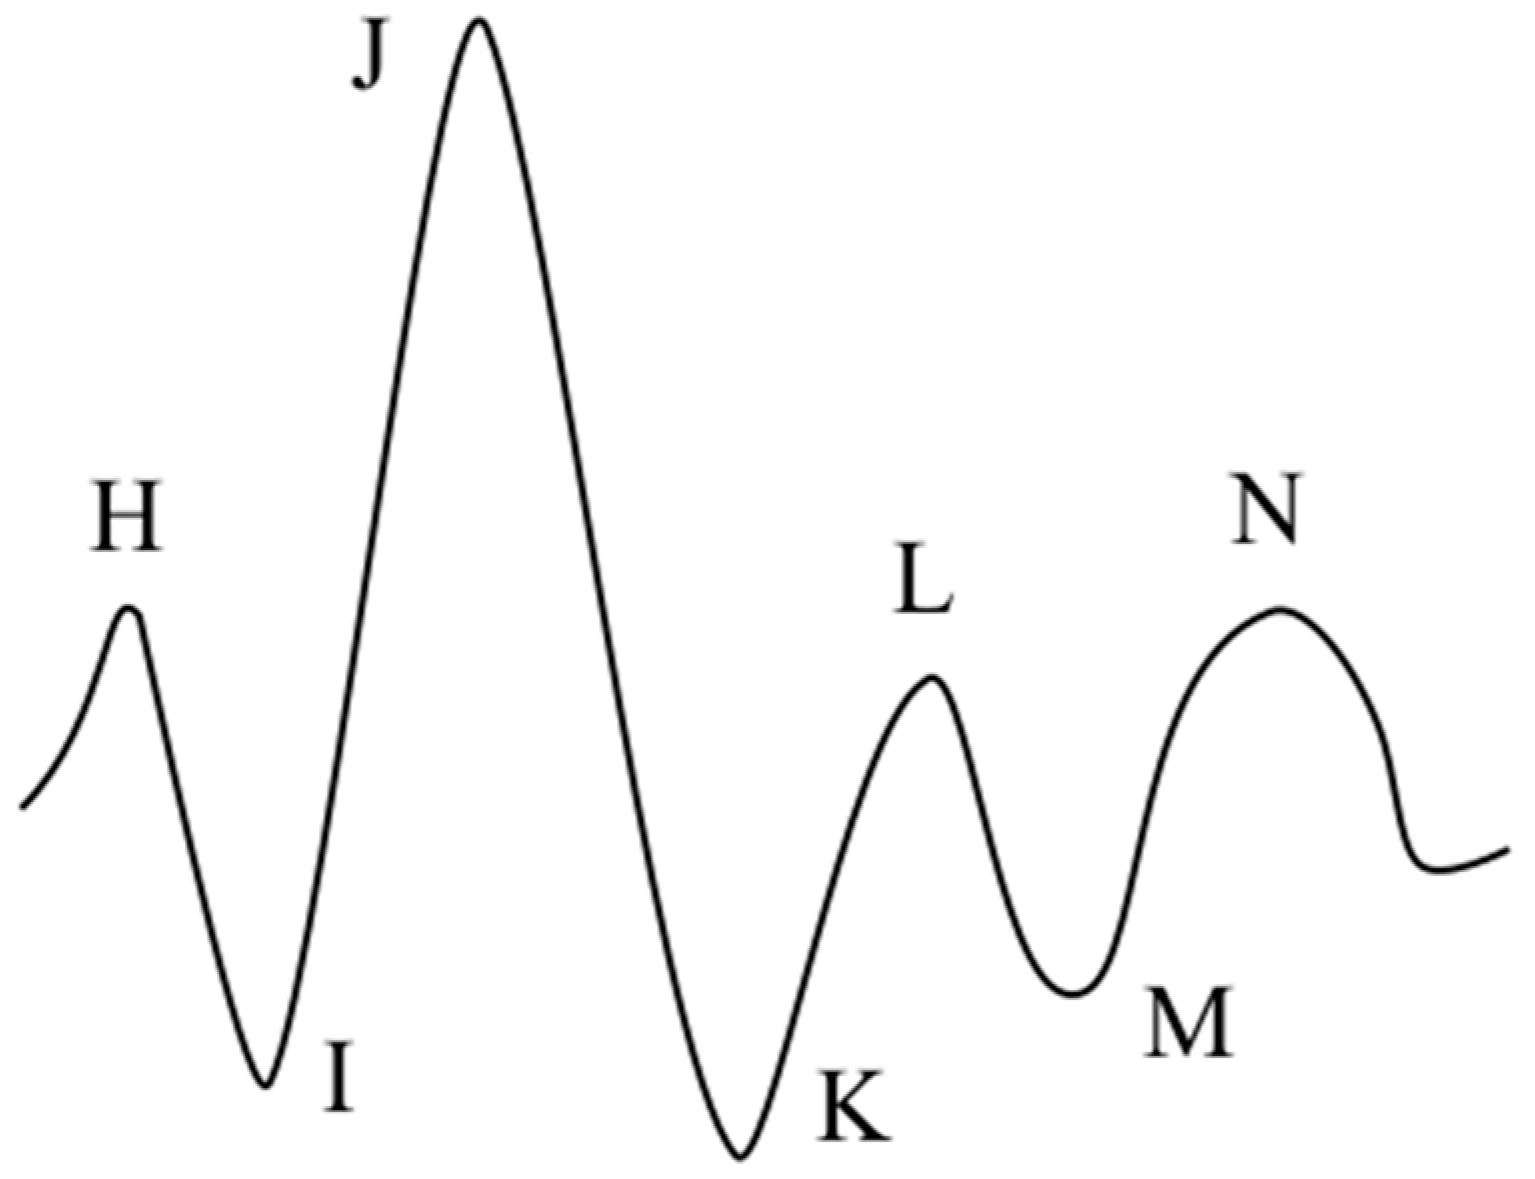
\includegraphics[width=0.7\textwidth]{pic/bcgWaveform.png}
	\caption[Beispiel eines typischen \ac{BKG}-Signals mit Nomenklatur]{Beispiel eines typischen \ac{BKG}-Signals mit Nomenklatur\protect\footnotemark}
	\label{fig:bcgwaveform}
\end{figure}
\footnotetext{Entnommen aus \cite{Albukhari2019} nach \cite{Starr1939}.}
